\chapter{Text Recognition Algorithms}

The root of any complex OCR software is text recognition. It is based on transforming an input image into its segmented form, with segments containing information about individual characters and their positions. In this chapter, we will analyze the individual steps that this process requires, along with a few obstacles the text recognition algorithms come across. These contribute to a poor quality of the given image and greatly impact the overall results. This leads to the conclusion that the software should behave according to them and try to solve these problems.

Firstly, we will therefore present the most common problems that lead to low image quality.

Secondly, we will demonstrate ways to solve them, which include image manipulation and the techniques of preprocessing. These try to minimize negative effects of poor quality images on text recognition algorithms.

Only once the preprocessing part is done can we move onto the actual recognition. This also consists of multiple steps. To detect characters or symbols in an image, we firstly need to segment the image into simpler parts that are easier to recognize. The individual techniques and types of segmentation, along with data representation are also thoroughly analyzed in this chapter. The last step of the algorithm discussed is actual character recognition from small segments and their transformation into a text format.

In this chapter, we also present an overview of some of the most popular optical character recognition software, including Tesseract, that is used in our implementation.

\section{Text Recognition Problems}

\xxx{meno tejto sekcie ok?}

Text recognition algorithms are most likely deemed to fail when the image presented is of low quality. This is because, similarly to the human eye, the software expects a significant difference between the characters and the background, expects parts of the images that represent the same character to look the same and is accustomed to working with aligned and properly straightened images.

In their paper,~\citet{preprocessAll} describe the following major difficulties that complicate the text recognition process:

\begin{description}
\item[Font face variability] Nowadays, a multitude of different fonts and styles is used in the documents. This includes different headers and footers, headings and body text, along with bold, italics and underlined characters, not to even mention differently colored fonts and even custom-made fonts. To hold the information about each and every one would be unsustainable for any OCR software, and, in case of custom-made fonts, even impossible, as there is currently no database of all existing fonts. Therefore, the OCR software needs to make assumptions and use heuristics to match its expectation of the character shape with the actual symbol it recognized.
\item[Handwritten text] Handwritten text is usually perceived as a type of more complicated font. On contrary to typical machine fonts, the characters that are supposed to be the same do not always have to look that way. This is why the OCR software has to count on minor character mistakes. These depend on different factors, such as line height, length, character size and others. Furthermore, handwriting can sometimes be unrecognizable even by a human eye. This case often prompts the software to fail.
\item[Scan quality] Poor scanning process or just poor initial image may cause suboptimal performance of the recognition algorithm. The image can be low-contrasted, not sharp enough, lines can be disrupted or pixelated (mostly in case of a low scan resolution), or it can contain a lot of noise. These problems are usually partly solved during the preprocessing part of OCR algorithm.
\item[Skew problems] Images that are skewed also come under the part of preprocessing. As the result of a scan or even a photography is almost never an image with a perfectly aligned text as it was on the paper, this needs to fixed, so the actual algorithm can count on correctly aligned images.
\item[Colors] As already mentioned before, OCR softwares work on the basis of distinguishing characters from the background. This leads to a simple observation --- the better the contrast of the image, the better the OCR results. Colored images generally have a lower contrast than when they are in black and white. Furthermore, there is no need for OCR software to keep the color information during the process, as it would only significantly complicate detection and increase time. Before passing to OCR, images therefore undergo binarization.
\item[Glyph similarity] Even people sometimes make mistakes when distinguishing characters like S and 5, O and 0, or I and l. OCR software can often make the same mistake, especially when handling documents that use various numbers of fonts \xxx{toto je ok?}, decorative fonts, or even  handwritten text.
\end{description}

These and multiple other factors are also the reason why the majority of OCR software works with `assumptions' about documents --- that the document has only one column, is not handwritten, that its lines are horizontally aligned and so on. Also, this is why no OCR software can work perfectly and will always keep encountering documents that are unrecoverable. 

However, there are many ways in which we can improve the results of the OCR. They either try to solve the already mentioned problems by processes like deskewing, image enhancement, denoising, or they simply increase the performance of OCR engines, like binarization. We will cover them thoroughly in the next section.

\section{Preprocessing}

Many of the existing OCR engines already come with some kind of built-in preprocessing filter. Their problem is that they most likely do not match the exact image case and are usually very simple.

This is why the best practice is to firstly preprocess the image and then pass the result to the OCR algorithm.

In this section, we will discuss the most important image transformations that we can perform to improve the results of the OCR. 

\subsection{Scaling}

OCR usually benefits from a properly scaled image with good resolution. It contains more detailed information that can be used to interpret text, which leads to higher accuracy of the result. This can be specifically applied to the case of resolution and bit-depth.

Many popular OCR engines (e.g. Tesseract~\cite{TesseractQual}, ABBYY FineReader~\cite{ABBYYdpi}) encourage their users to use 300 dpi images. Their reason for that is pretty simple --- it is the point where they gain the most accuracy without sacrificing speed and file size~\cite{preprocessAll}. Another reason for the use of 300 dpi is the fact that most OCR engines are trained to this resolution. Some engines (like the already mentioned ABBYY FineReader~\cite{ABBYYdpi}), no matter what resolution you give them will actually sample up or down to get to 300 dpi. 

Obtaining a 300 dpi scan using currently available hardware is simple enough. However, if the user has already provided us with an image of a different resolution, our next step is to either upscale (if the dpi of the input image was lower) or downscale (if the dpi of the input image was higher) the image. In both cases, a technique called \emph{interpolation} is used. 

Interpolation works by using known data to estimate values at unknown points. It specifically approximates the resulting pixel's color and intensity based on the values at surrounding pixels. When downscaling, this technique therefore computes one color value for each set of pixels, which are the color values of the pixels in the new image. When upscaling, it computes color values of the new pixels by approximating the values of the old pixels around them.

This technique tries to minimize the aliasing effect of the resulting image --- so the scaled picture does not appear visibly pixelated and it's edges are not jagged.

Interpolation algorithms can be grouped into two categories: \emph{adaptive} and \emph{non-adaptive}.

\emph{Adaptive methods} change the way they treat various pixels depending on what they are interpolating, specifically smooth texture vs. sharp edges. They are primarily designed to minimize the presence of interpolation artifacts in regions where they are most apparent, and they differ by the way they detect edges.

\emph{Non-adaptive} methods, on the other hand, treat all pixels equally. Their complexity depends on the number of adjacent pixels during interpolation, which is also the criterion by which the existing methods are classified~\cite{interpolation}. We present these methods in~\cref{fig:preprocessInterpolation}.

\begin{figure}[t]
\centering
{\sffamily
\begin{tabular}{cc}
Original & Nearest-neighbor Interpolation\
 & (1 pixel) \\
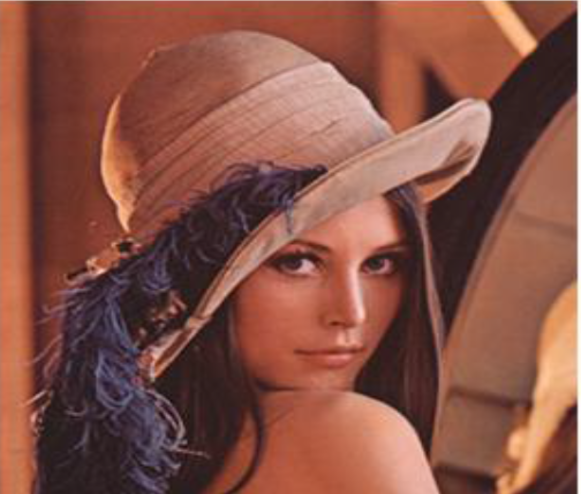
\includegraphics[width=.4\linewidth]{img/preprocessing/interp_orig.png}
&
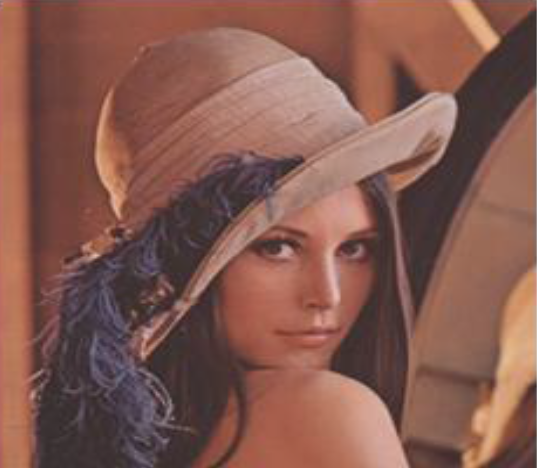
\includegraphics[width=.4\linewidth]{img/preprocessing/interp_nn.png}
\vspace{1em} \\
Bilinear Interpolation & Bicubic Interpolation \\
($2\times2$ pixels) & ($4\times4$ pixels) \\
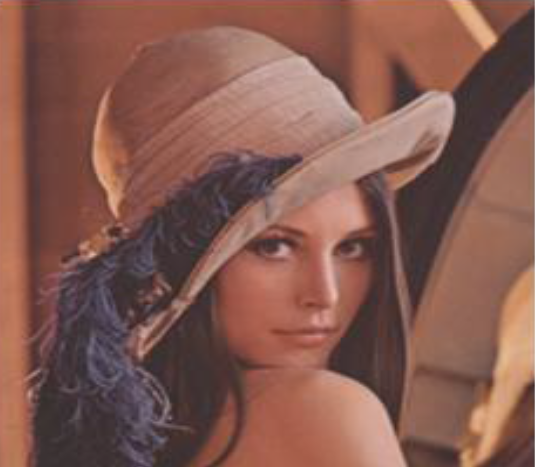
\includegraphics[width=.4\linewidth]{img/preprocessing/interp_bili.png}
&

\includegraphics[width=.4\linewidth]{img/preprocessing/interp_bicubic.png}
\end{tabular}
}
\caption{Non-adaptive methods of Interpolation}
\xxx{ten 1 pixel chcem mat pod nearest-neighbor}
\label{fig:preprocessInterpolation}
\end{figure}

There also exist higher order interpolations, such as \emph{Spline}, \emph{Sinc}, \emph{Lanczos} or \emph{Discrete Wavelet Transforms}~\cite{interpolation}. These consider more surrounding pixels and calculate the resulting value through more complex functions, like transforms or sampling functions. The results are more accurate than those of simple calculations at the cost of significantly more time. For the purposes of OCR, such complex and time-consuming functions are not desirable, as we are not yet working with any rotations and distortions and just need to resize the existing image.

For the best quality/time ratio, the popular decision in most cases is \emph{Bicubic Interpolation}. Although \emph{Neareast Neighbor} and \emph{Bilinear} methods are extremely fast, the results were found to be poor~\cite{interpolationComp}.

\subsection{Binarization}

To recognize characters in an image, an OCR software must distinguish the background pixels from the actual pixels that belong to the characters. The software must therefore divide all the existing pixels of the image into two groups --- a background group and a symbols group. To determine the boundary between them is a complex task when it comes to colored images, as we need to process the whole RGB information of each pixel. However, when it comes to grayscale images, we obtain only one value. Moreover, monochrome one images contain pixels of only two values --- black and white --- which make the process of finding a boundary trivial.

This is why it is beneficial for images to undergo the process of binarization, which converts images into their monochrome one form.

Many binarization algorithms work under the assumption that the input image is already in grayscale. If not, they firstly transform the image to grayscale, then apply the binarization techniques.

\subsubsection{Grayscale conversion}

\emph{Grayscale conversion} is the process of computing and assigning a gray value for each colored pixel from its attributes. There exist a few different approaches to this problem. The simplest one is the \emph{averaging approach}, which assigns each pixel the average of its R, G and B value. However, this does not really reflect the way human eye perceives colors. Our perception of colors is non-uniform --- green color is perceived more strongly than red, and red more strongly than blue. For this reason, a correction formula (often called \emph{luma}~\cite{grayscaleConv}) that weights each color component differently is used. We present these techniques in~\cref{fig:preprocessGrayscale}.

Another way to approach grayscale conversion is to represent the color based on its HSL values and convert it to its least saturated variant.

As decribed by~\citet{grayscaleCadik}, these exist many more algorithms approaching this problem. Most of them require more complicated computations and try to preserve attributes of the image that may be lost during the process --- like contrast or luminance.

\begin{figure}[t]
\centering
{\sffamily
\begin{tabular}{ccc}
Original & Averaging technique & Luma correction \\
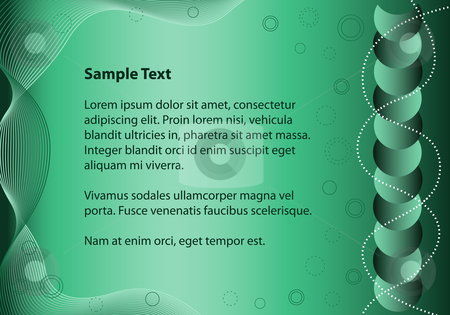
\includegraphics[width=.28\linewidth]{img/preprocessing/grayscale_orig.jpg}
&
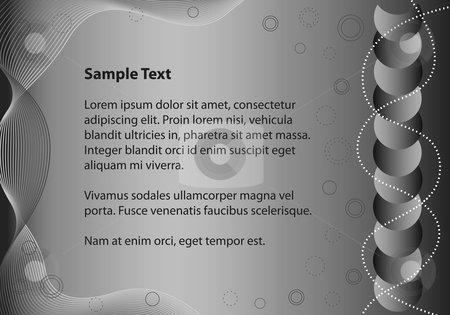
\includegraphics[width=.28\linewidth]{img/preprocessing/grayscale_avg.png}
&
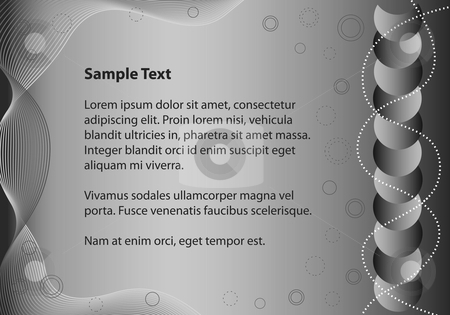
\includegraphics[width=.28\linewidth]{img/preprocessing/grayscale_luma.png}
\end{tabular}
}
\caption{Comparison of grayscale techniques}
\label{fig:preprocessGrayscale}
\end{figure}

\subsubsection{Threshold-based binarization}
Once the image is in grayscale mode, the next step is to binarize it. Binarization methods work on the basis of a \emph{threshold} --- a set value that a pixel is compared to. If it is greater than the threshold, it is assumed to be white, otherwise, it is colored black. Various binarization methods differ in the way that this threshold is calculated and used.

The simplest approach to binarization is \emph{global thresholding}~\citep{globalThresh}. It works by choosing a threshold value and iterating over the whole image, comparing the value of each pixel to this threshold. If it is greater, the pixel in the resulting image will be black, otherwise white. However, as the brightness and contrast of different images vary, it is impossible to choose a threshold suitable for all images.

More complex methods that aim to correct the problems of global thresholding exist. Some of these include:
\begin{itemize}
\item Otsu's method for global threshold estimation~\citep{otsu}
\item Local-thresholding methods~\citep{localOtherBin}:
\begin{itemize}
\item Niblack method
\item Bernsen method
\item Sauvola method
\end{itemize}
\end{itemize}

Otsu's method statistically computes a global threshold by a dynamical classification of image pixels into background and foreground pixels. Although simple and easy to implement, but, as any global method, it is inherently unable to fix high variance or uneven spots in an image background. Local-thresholding methods aim to solve this issue by allowing different threshold values in different parts of the image. They differ in the way the existing thresholds are computed --- for example, Niblack's method~\citep{adaptiveBin} uses mean and standard deviation of surrounding pixels for each pixel, Sauvola Method improves it by checking for blank regions and Bernsen's method by optimizing Niblack's computations. 

Visual differences between the mentioned methods are displayed in~\cref{fig:preprocessBinarization}. Comprehensive reviews of other, more complex methods are available~\citep{localOtherBin}.

\begin{figure}
\centering
{\sffamily
\begin{tabular}{ccc}
Original scanned image &
Global Thresholding &
Sauvola Binarization \\
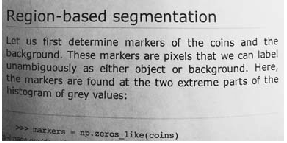
\includegraphics[width=.3\linewidth]{img/preprocessing/bin_orig.png} &
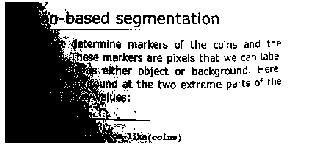
\includegraphics[width=.3\linewidth]{img/preprocessing/bin_glob.png} &
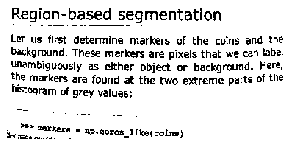
\includegraphics[width=.3\linewidth]{img/preprocessing/bin_sauvola.png}
\end{tabular}
}
\caption{Comparison of binarization method output on an unevenly lit image}
\label{fig:preprocessBinarization}
\end{figure}

\subsection{Contrast enhancement}

Another important factor that results in low-quality images is low contrast. Even human eye has a harder time recognizing images with this element. The same stands for OCR engines, as low contrast often results in possible blending of edges during recognition.

An image \emph{histogram} is used to improve this aspect. A histogram is an accurate representation of the distribution of data and, in case of image histograms, it represents the tonal distribution of an image --- x-axis stands for all available tonal levels, and y-axis represents the number of pixels for each tonal level. In colored (RGB) images, the histogram is displayed by the terms of three separate histograms --- one for each color component.

Contrast of the current color component is represented as distribution of pixel luminance values. By spreading out the most frequent intensity values of the histogram, the contrast of the image increases(~\cref{fig:preprocessContrastComparison}).

\begin{figure}[t]
\centering
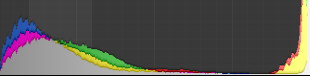
\includegraphics[width=0.4\linewidth]{img/preprocessing//histogram_low.png}
\qquad
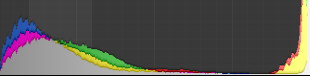
\includegraphics[width=0.4\linewidth]{img/preprocessing/histogram_high.png}
\caption{Image histogram. Left: low contrast image histogram, right: high contrast image histogram.}
\label{fig:preprocessContrastComparison}
\end{figure}

To expand the original digital values of histogram into a new distribution, different histogram spreading methods use functions of different forms. These can be either linear or non-linear, which leads to the categorization of histogram spreading methods into either \emph{linear stretching} methods or \emph{non-linear stretching} methods~\citep{linearNonStretch}.

Both types of methods have their advantages and disadvantages. Although linear methods are easier to implement, non-linear methods were shown to have given better performance~\citep{chandpa1comparative} and overall better results. Linear methods still produce satisfactory results on remotely sensed images with Gaussian or near-Gaussian histograms, and in contrary to non-linear methods, objects in the original scene do not lose their correct brightness value.

For contrast enhancement of the text, a non-linear technique called \emph{histogram equalization}~\citep{histogramEQ} is used. Is is based on transforms that depend on the probability distribution function of the histogram. Although it produces unrealistic and over-enhanced effects in photographs, the over-processing actually suits the text data. We present the effects of this widely used method in~\cref{preprocessHistogramEqualization}.

Many other more complex and complicated techniques of contrast enhancement exist. These were presented by~\citet{contrastOther} and contain techniques like CLAHE, Dynamic Stochastic Resonance and generic transforms, such as Fourier, Discrete Cosine, and Wavelet. For complex text recognition cases, CLAHE method can be used with satisfactory results.

\begin{figure}[t]
\centering
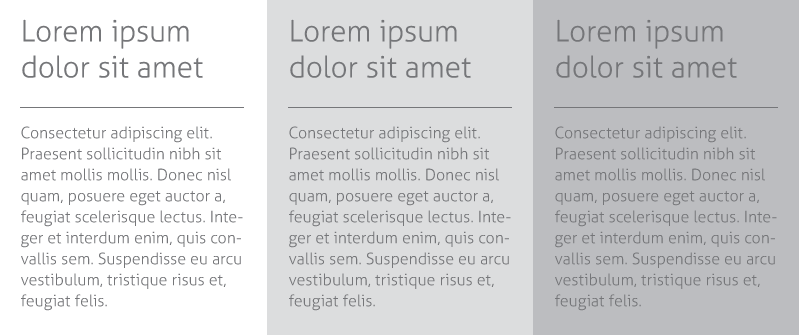
\includegraphics[width=0.4\linewidth]{img/preprocessing/contrast_low.png}
\qquad
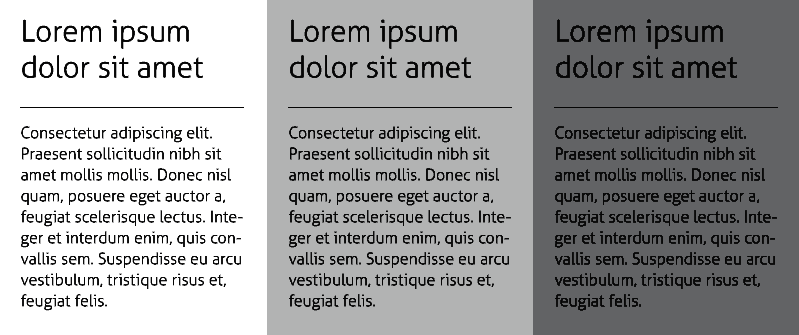
\includegraphics[width=0.4\linewidth]{img/preprocessing/contrast_high.png}
\caption{Histogram equalization. Left: original image, right: processed image.}
\label{fig:preprocessHistogramEqualization}
\end{figure}


\subsection{Deskewing}

Skewed images are probably the most common problem that many OCR engines struggle with. They usually appear when an image is scanned or photographed crookedly. 

One of the steps of OCR algorithms is \emph{page segmentation}. It is the process that decomposes a document image into elements. This division is based on vertically and horizontally aligned characters, spaces and other artifacts. We will discuss this topic thoroughly in the following chapter. For now, the important thing to know is that skewed images pass misaligned data to the OCR algorithm. This causes more errors and ultimately leads to poorer results.

There are different approaches that deal with this problem. All of these methods work (for more accurate results) after binarization of the image and generally assume the skew angle to be no more than 15$^{\circ}$. Algorithms that work on greater skew angles also exist~\citep{skewAngleDetection}. They are not as widely used, though, as most of the time, correction needs to be done on scanned documents --- which are mostly only slightly tweaked.

The most effective and popular algorithms include the following~\citep{skewBestTechniques}:
\begin{itemize}
    \item Hough Transform
    \item Projection Profile method
    \item Cross Correlation
    \item Connected Component Clustering (or \emph{Nearest Neighbor Clustering})~\citep{skewClustering}
\end{itemize}
However, worth noting are also other methods like \emph{Fourier}~\citep{fourierTransform}, Wavelet Decomposition, Radon Transform, PCP, one-pass or multi-pass skew correction, morphology algorithms\ldots.. 

The above mentioned methods differ in the way they determine the skew of the image. Hough transform applies feature extraction to the image and assigns the skew of the line with the most number of pixels to the document. Projection profile method rotates the image and finds the skew where its histogram along horizontal scan lines has the most peaks and valleys, while the cross correlation method uses this method and applies it to multiple vertical segments. Moreover, connected component clustering method is based on finding the coherency between connected components of the image and determining their common skew. We present the advantages and disadvantages of these methods in~\cref{tab:preprocessSkewProsCons}.

\begin{table}[t]
{\small
\begin{tabular}{p{5em}p{13em}p{13em}}
\toprule
\textbf{Method} & \textbf{Advantages} & \textbf{Disadvantages} \\
\midrule
Hough Transform
&
- highly effective
&
- time consuming

- cannot obtain data from graphics in an image, therefore ineffective at their presence

\\
Projection Profile method
&
- easy to implement

- works well on images with skew under 10$^{\circ}$
&

- fails at the presence of graphics

- computationally expensive

\\
Cross Correlation
&

- better time complexity than projection profile method

- needs less data with no loss in accuracy

&

- works on text areas only

- fails at the presence of graphics

\\
Connected Component Clustering
&

- satisfactory results for skew up to 20$^{\circ}$

- generally work well in non-text areas

&

- low quality images deem the method to fail

- clustering algorithm needs to be picked carefully to avoid errors

\\
\bottomrule
\end{tabular}
}
\caption{The advantages and disadvantages of different deskewing methods}
\label{tab:preprocessSkewProsCons}
\end{table}

\begin{figure}[t]
\centering
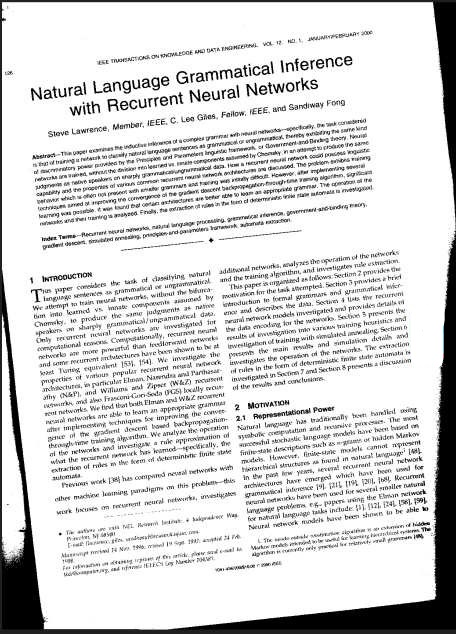
\includegraphics[height=0.25\textheight]{img/preprocessing/deskew_orig.jpg}
\qquad
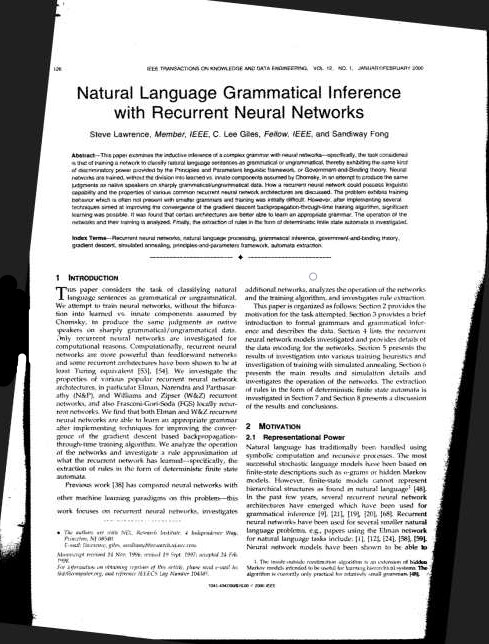
\includegraphics[height=0.25\textheight]{img/preprocessing/deskew_new.jpg}
\caption{Image deskewing illustrated. Left: original image, right: deskewed image.}
\label{fig:preprocessDeskewing}
\end{figure}

\subsection{Noise reduction}

Image noise is an usually unwanted random variation of brightness or color information in images, reminding film grain in digital cameras. It is often caused by the sensor of a scanner or a digital camera attempting to record small amounts of light. 

For OCR engines, processing noise can be quite tricky. Its presence is especially crucial during binarization and edge detection. These processes are based on the differences between the "outside" of the element and its "inside". When noise is present, it can disrupt these borders, which can often cause the failure of recognition. We present the different types of existing noise in~\cref{tab:preprocessNoiseTypes}.

\begin{table}[t]
{\small
\begin{tabular}{p{8em}p{12em}l}
\toprule
\textbf{Type} & \textbf{Description} & \textbf{Image} \\
\midrule
Salt and Pepper \par (\emph{impulse noise})
&
Randomly occuring black and white pixels caused by sharp and sudden
disturbances in image signal present in old photographs.
&
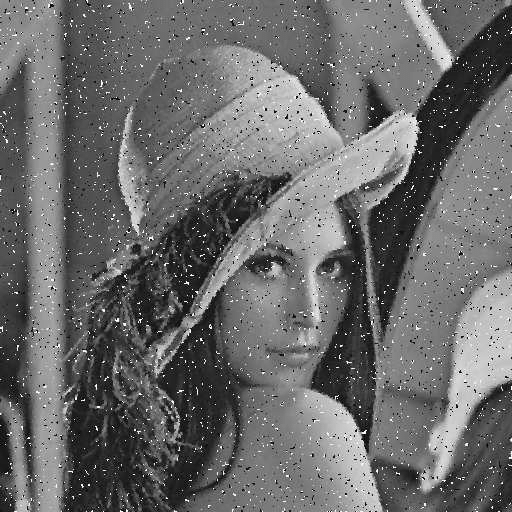
\includegraphics[width=0.3\textwidth, align=t]{img/preprocessing/noise_saltpepper.png} \\
Statistical noise 
&
Unexplained variability whithin an image, usually characterized by a probability density function, e.g.~\emph{Gaussian noise}, \emph{Shot noise}, \emph{Quantization noise} or film grain.
&
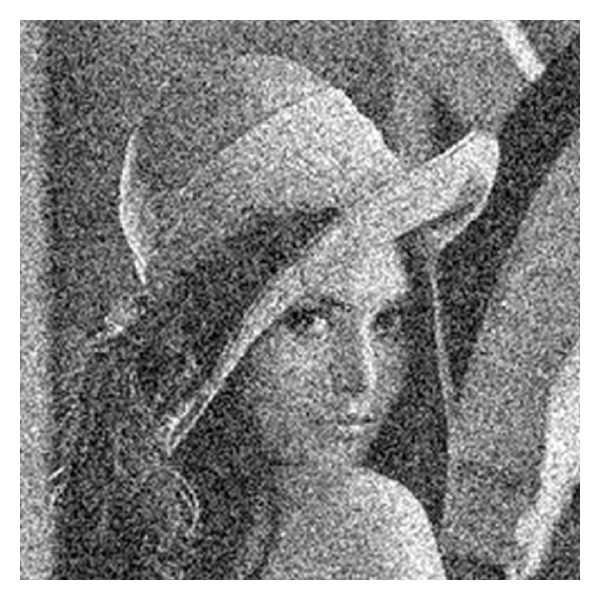
\includegraphics[width=0.3\textwidth, align=t]{img/preprocessing/noise_gaussian.jpg}\\
Other
&
E.g.~\emph{anisotropic} or \emph{periodic} noise, often found in old photographs or documents.
&
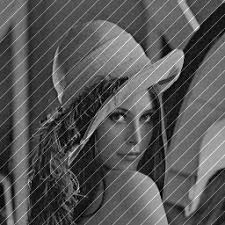
\includegraphics[width=0.3\textwidth, align=t]{img/preprocessing/noise_periodic.jpg} \\
\bottomrule
\end{tabular}
}
\caption{Different types of noise}
\label{tab:preprocessNoiseTypes}
\end{table}

When performing noise reduction, common image processing filters are used~\citep{denoisingTechniques}. These can be categorized as either \emph{linear} or \emph{non-linear}, depending on their linearity relationships.

Linear filtering, such as \emph{mean filtering}, \emph{Gaussian filtering} or \emph{Wiener filtering}, is a filtering in which the value of an output pixel is a linear combination of the values of the pixels in the input pixel's neighborhood. When used for noise reduction, they work on averaging the color values of neighbour pixels, so they can help assure an averaged view of the contrast along regions of different color. This, however, rather than correcting the color of the affected pixel, results in creating an area with an average (and incorrect) color. This blurs the edges and smooths out other fine details. They are still widely used, though, as they require only a small amount of computations, which leads to increased speed and easy and simple implementations.

Non-linear filtering, on the other hand, renders an output which is not a linear function of its input. In noise reduction, one of the most popular filter in this category is a \emph{median filter}. It works similarly to a mean filter, but for each pixel, instead of replacing its value with a mean of surrounding pixels, it calculates the median. In comparison to linear filters, it provides considerably sharper images and in most cases preserves the edges. The downside is the increased run time, and with high level of noise, results are almost the same as with linear filters. However, it is highly effective on salt and pepper noise.

\item Worth mentioning is also \textbf{non-local means method} \citep{nonLocalMeans}. It is based on taking a mean value of all pixels of the image, weighted by how similar these pixels are to the target pixel. This technique produces an even sharper and clearer image results as mentioned filters. However, it comes with the expense of additional increased speed.


\begin{figure}
\centering
{\sffamily
\begin{tabular}{cc}
Original & Gaussian filter \\
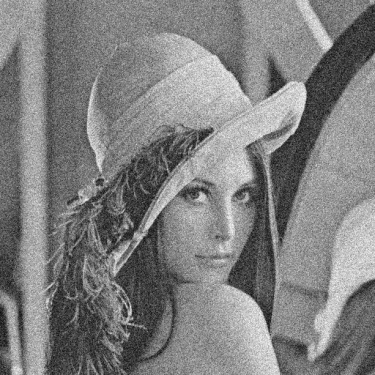
\includegraphics[width=.4\linewidth]{img/preprocessing/denoise_orig.png}
&
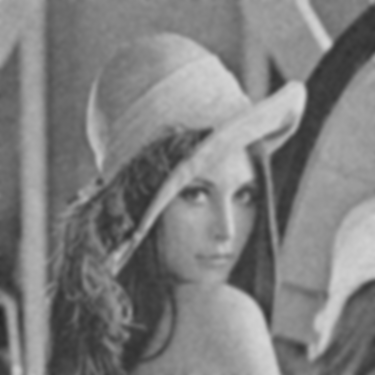
\includegraphics[width=.4\linewidth]{img/preprocessing/denoise_gauss.png}
\vspace{1em} \\
Median filter & Non-local means method \\
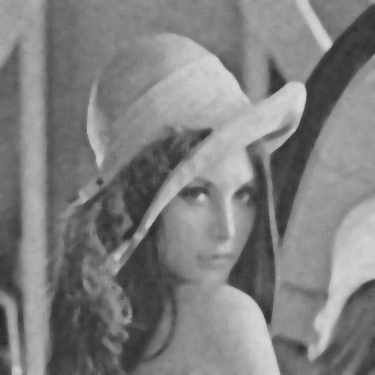
\includegraphics[width=.4\linewidth]{img/preprocessing/denoise_median.png}
&
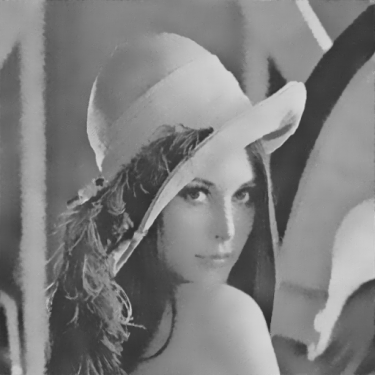
\includegraphics[width=.4\linewidth]{img/preprocessing/denoise_nonlocal.png}
\end{tabular}
}
\caption{Comparison of denoising techniques.}
\label{fig:denoising}
\end{figure}

What combination of techniques to use for the optimal results greatly depends on the input image --- if there is little to no noise, de-noising an image can cause more harm than good. Therefore, it is always important to approximately compute the signal:noise ratio before applying any kind of filters.

\xxx{Je toto dalej vobec potrebne? Mozno by som napisala len nieco ako ze toto zratat je fakt tazke, niektore komplikovane metody na to existuju (citacia), no casto maju blbe vysledky, preto to OCR engines nepouzivaju a promptuju uzivatela to radsej spravit sam}

To calculate this properly is a more complex task than thought. Although simple algorithms have already existed for a few years, they return poor results and most of them are almost not worth using because of the time complexity. They are mostly based on comparison - testing the difference between each pixel and its neighbors for various threshold numbers based on the dynamic range and calculating deviation, picking "windows" of different sizes and calculating their means and deviation, based on which we decide whether the center pixel is corrupted or not and so on\ldots

For a more complex (and sufficient) solution, we have to run many more mathematical calculations on the input image \citep{noiseDetection}. These calculations require a lot of knowledge in the field of probability and statistics, specifically probability distribution. The basic idea for these noise recognition algorithms is \emph{separating frequencies}. This is usually done by dividing the image into blocks and running a transformation (for example a \emph{discrete cosine transformation}) on each of the blocks. The frequency components are then grouped by increasing frequency. Then, the extraction of statistical features (such as kurtosis, mean, standard deviation) is performed.

Noise is most likely to be found on higher frequencies and we use this observation along with our computed statistical features to determine the thresholding on higher frequencies. If the threshold of the input image is greater, the image is determined to be noise-free. 

\subsection{Scanning border reduction}

Scanned documents often have visible dark borders (\emph{marginal noise}). These are created either during scanning (due to the presence of neighbouring pages) or are an unwanted result of the binarization process.

As performing a scanning border removal might be harmful in case there was no marginal noise present, this process has two steps --- marginal noise detection and, if successful, marginal noise reduction.

Marginal noise is present as a dark connected component of the page. This is a fact that most detection algorithms take advantage of. Firstly, they extract the connected components of the page. This can be done for example by a \emph{black filter} (a moving rectangular window that calculates the ratio of black pixels on border~\citep{marginalNoiseWindow}). After obtaining the connected components, different heuristics are used --- most based on removing the connected components near the edges. In the end, usually a "cleanup" is performed (like \emph{white filter}~\citep{marginalNoiseWindow}) for removal of all unnecessary elements around the borders (an unwanted text from the neighbour page, noisy components in the corners\ldots).

The results of this algorithm depend greatly on the values of thresholds, margins and other hard coded parameters. This is why the cleanup part's parameters are usually dependant on the results of previous parts of this process.

Another approach is the one mentioned by \citet{marginalNoiseEdge}. It is based on edge density calculations, and the fact that text areas have generally a much lower density than edge areas. An edge detector (in this case, \emph{sobel}) is used for examining vertical marginal noise, and later horizontal marginal noise. It returns the positions of the margins. Anything beyond these positions is detected as an unwanted noise, and can be therefore removed by filters or other removal algorithms.

\begin{figure}
\centering

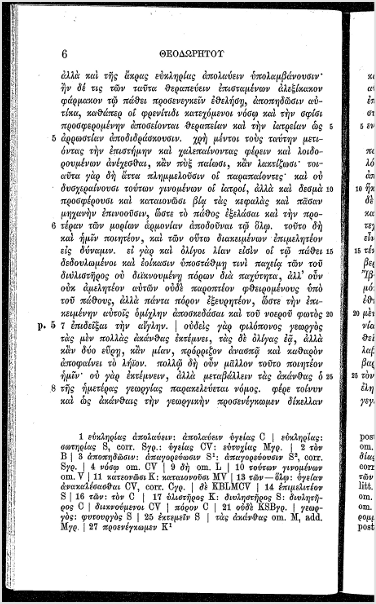
\includegraphics[height=10em]{img/preprocessing/scan_borders_orig.png}
\qquad
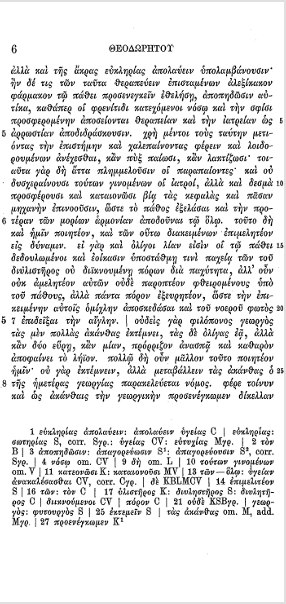
\includegraphics[height=10em]{img/preprocessing/scan_borders_result.png}

\caption{Removal of scanning artifacts. Left: original, right: removed scanning borders.}
\label{fig:scanning}
\end{figure}

\section{Text detection process}

Nowadays, two approaches are proposed for text detection in OCR. The first one is an approach based on heuristics --- page segmentation, line and element detection and only after that, character detection, which is based on different approximations and sometimes naive algorithms. The second one is an approach that is widely used and researched today --- and that is the use of neural networks.

In this paper, we will be concentrating on the heuristics approach of the OCR problem, as we use it in our implementation. However, neural network recognition is nowadays an approach returning \xxx{?? spravne?} promising results and also deserves a mention.

A lot of OCR engines differ in the way their heuristic approaches work. They all agree on one thing, though, and that is the succession of steps that need to be implemented. Firstly, a \emph{page segmentation} has to be performed. This divides the given page into multiple segments that are easier to process when determining the elements of the image. Now, the recognition algorithm could simply take place. However, most of the existing OCR engines (like Tesseract) "pre-process" the output of page segmentation. They use steps like \emph{representation} and \emph{feature extraction}, which are based on simplifying the extracted elements of image documents. This contributes to better results of the OCR, and, last but not least, helps to improve the speed of the algorithm.

Only after this, the character recognition algorithm is applied.

We will analyze these steps in the following individual subsections.

\subsection{Page Segmentation}

In many cases, OCR system heavily depends on the accuracy of page segmentation process \citep{pageSegmentation}. There are three main approaches \citep{segmentationBenchmark} to this problem --- either we start with an image as a whole and recursively divide it into parts until criterion is met, or we start with individual pixels and group them according to similarity of their attributes, or we use a combination of these two methods. Based on these methods, there exist a few concrete algorithms widely used for heuristic page segmentation.

\subsubsection{Page Segmentation Techniques}

\xxx{TO DO - chcem dat captions tym fboxom, netusim vobec ako}

\clearpage

\begin{longtable}{p{7em}p{13em}c}
\toprule
\textbf{Page} & \textbf{Description} & \textbf{Image} \\
\textbf{Segmentation} & & \\
\textbf{Algorithm} & & \\
\midrule
RXYC

algorithm

(\emph{X-Y cut})
&

one of the oldest and simplest methods

tree based algorithm, works by recursively splitting the nodes of the tree into rectangular parts

uses projection profile and threshold computations for determination of splitting

easy to implement, fast

usually fails at the presence of imperfections

&
\fbox{\raisebox{-\height}{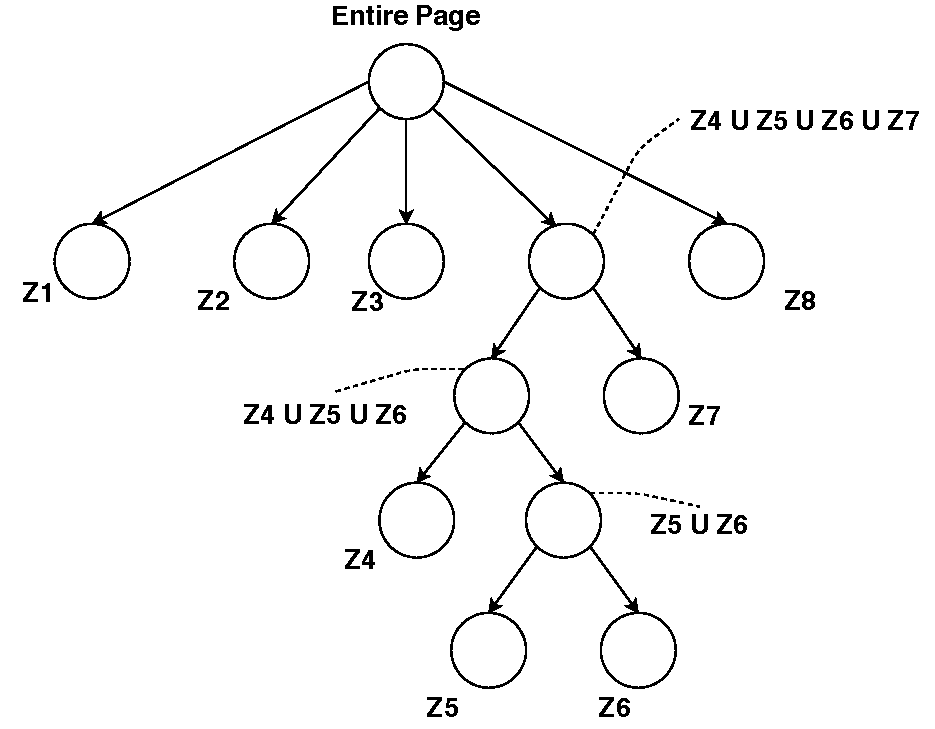
\includegraphics[width=0.3\textwidth,
height=40mm]{img/textDetection/segm_rxyc.pdf}}}\\
Smearing 

algorithm 

(\emph{RLSA})
&

based on linking together black areas that are no more than C pixels away from each other

requires binarized images

slightly better results than \emph{X-Y cut}

fails at the presence of noise, not used for text documents

widely popular among vehicle plate recognition
 &
\fbox{\raisebox{-\height}{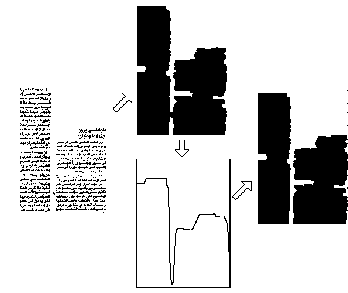
\includegraphics[width=0.3\textwidth,
height=40mm]{img/textDetection/segm_smearing.png}}}\\
Voronoi

diagram 

based

algorithm&

bottom-up algorithm

performs a noise removal 

creates Voronoi diagram from sample points of edges of extracted connected components of the existing image

performs a "clean-up" of the diagram - deletion of superfluous edges

can be used on documents with noise and other imperfections

causing over-segmentation errors when working with documents using different fonts or styles

advised to use on homogeneous collection of documents &
\fbox{\raisebox{-\height}{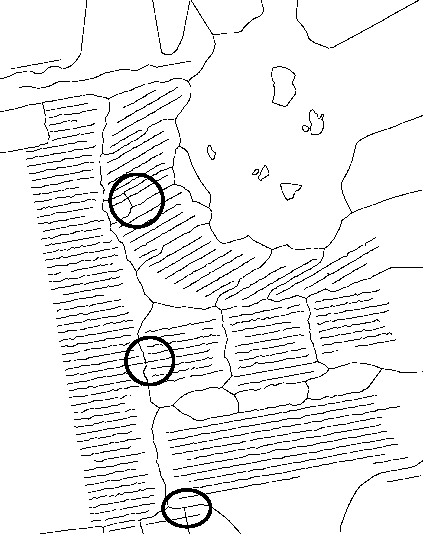
\includegraphics[width=0.3\textwidth,
height=60mm]{img/textDetection/segm_voronoi.png}}}\\
Docstrum

algorithm

&

bottom-up algorithm

based on fonts and styles of the characters

divides connected components into a dominant font group and a group with characters from titles or sections heading

performs a near-neighor clustering of components in each group

determines the skew of the image and text-lines, upon which merges within-line nearest neighbor pairs into text-lines and blocks

similar errors like \emph{Voronoi diagram} algorithm

advised to use on a homogeneous collection of documents
&
\fbox{
\raisebox{-\height}{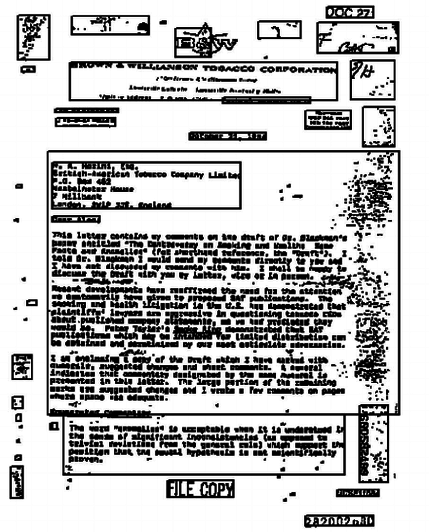
\includegraphics[width=0.3\textwidth,
height=60mm]{img/textDetection/segm_docstrum.png}}}\\
Whitespace

analysis

&

assumes a white background of the image

finds a union of white rectangles as a cover of the background

uncovered regions of the image after applying the union are the results of segmentation

satisfactory results on heterogeneous documents

tends to result in either over-segmentation or under-segmentation depending on the sizes of rectangles in the union

overall, performs worse than \emph{Voronoi} or \emph{Docstrum} algorithm
&
\fbox{
\raisebox{-\height}{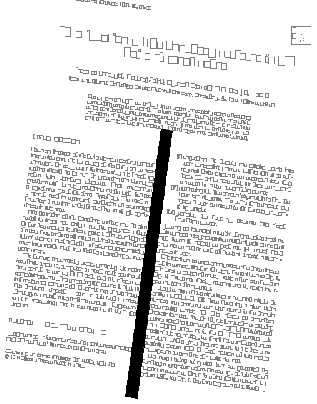
\includegraphics[width=0.3\textwidth,
height=60mm]{img/textDetection/segm_whitespace.png}}}\\
Constrained

text-line

detection
&

similar to \emph{whitespace analysis}, differs in the approach of finding the whitespace rectangles that cover the page background

good option for documents with different font sizes or layouts

nearly parameter free
&
\fbox{
\raisebox{-\height}{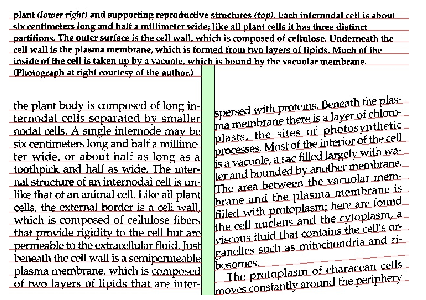
\includegraphics[width=0.3\textwidth,
height=60mm]{img/textDetection/segm_textline.png}}}\\
\bottomrule
\caption{Page Segmentation Algorithms}
\label{tab:page_seg_algorithms}
\end{longtable}

\subsubsection{Tesseract page segmentation}

Another slightly different segmentation technique was proposed by \citet{tesseractSegmentationTab}. This method is based on detecting so-called \emph{tab-stops}.

\emph{Tab-stops} are used in word processors to enable correct and eye pleasing alignment of text, and are present in the document as margins, column edges, indentations. All of them are placed at fixed x-positions at which edges or centers of text lines are vertically aligned. This process has multiple steps. Firstly, it preprocesses the document image for connected components. By grouping these connected components into vertical lines and examining their vertical alignment, tab-lines are then detected, which mark the text-lines with their beginning and end. Based on these tab-lines, connected components of the page layout analysis are then grouped into \emph{column partitions}, which do not cross any tab-lines and are of the same type. In the end, a few of the column partitions can be merged or divided into segmented blocks, based on different types of fonts or line spacing. 

This method is implemented and used by the Tesseract engine, with the preprocessing help of the Leptonica library. It claims to yield satisfactory results, given the input document is properly preprocessed.

As our implementation uses the Tesseract engine for symbol recognition, this is also the method of page segmentation that it uses.

\begin{figure}
    \noindent
	\makebox[\textwidth]{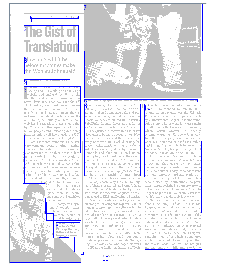
\includegraphics[width=20em]
	{../img/textDetection/segm_tabstop.pdf}}
	\caption{Tesseract Engine Segmentation}
	\label{fig:mff}
\end{figure}

There exist many other segmentation methods that approach this problem differently. For example, with segmentation of scanned books that mostly have Manhattan layout, a simple deskewing and horizontal and vertical cuts should suffice. Also, algorithms focusing on recipe or ticket analysis already know what the approximate layout of the received image will be. They can therefore simplify these complicated algorithms for their purposes.

\subsection{Representation and feature extraction}

Upon extracting elements by page segmentation, we are left with an unnecessary amount of information. We could feed all of them into a recognizer. This would, however, decrease accuracy of recognition and significantly increase its time complexity. For these reasons, a set of features is extracted for each element that distinguishes it from other element classes while keeping characteristic differences. There exist various different features, generally divided into local features, which are usually geometric (like number of endpoints of each character, convex or concave parts, branches etc.), and global features, which are usually topological (connectivity, number of profiles, number of holes\ldots). The set of features that will represent each characters needs to be picked carefully, so that they define the shape of a character precisely a uniquely but are also the smallest set possible to prevent increased memory usage and time complexity.

There exist three methods for performing feature extraction, described by both \citet{featureExtractionBook} and \citet{featureExtractiontext}. They differ in the ways the features are derived from the character, in reconstructability (whether the image can be reconstructed to its previous version solely from its features), in invariance to transformations and many more. We describe these methods in the following list:

\begin{itemize}

\item \textbf{Global transformation and series expansion} \todo{proc bold?} \xxx{nejak som chcela dat nadpis tomu itemu a toto vyzera ze to tak zvyraznuje, mam dat emph?}:

These include methods like Fourier or Gabor transform, Fourier Descriptor, Wavelets, Moments and Karhunen-Loeve expansion, and are based on the representation of continuous signals by a linear combination of simpler functions. The coefficients of the linear combination provide a compact encoding known as transformation or series expansion. Therefore, deformations like translation and rotations are invariant under global transformation and series expansion. However, the downside of this approach is the time complexity, as this method requires a number of non-trivial computations {\xxx{calculations?}}.

\item \textbf{Statistical representation}

Unlike transforms, these features are based on the statistical distribution of points in the element. They provide high speed and low complexity and also take care of different font and style variations to some extend. Methods based on this representation are e.g. \emph{zoning} (where the frame containing the character is split into different zones, which are then analyzed for densities of points and strokes), \emph{crossings and distances} (crossing --- the number of crossings of the character along vertical and horizontal lines; distances --- the distances of character pixels from frame boundaries), and other like projections, characteristic loci etc. 

The downside of this approach is the invariance to transforms --- if the character is only slightly skewed, the feature extraction results will greatly differ.

\item \textbf{Geometrical and topological representation}

These features are based on the basic line type that form a character skeleton, extracting features of the character contour like extreme points, maxima, minima, cross points, line ends, isolated dots, different types of strokes and many more. These feature have high tolerances to distortions and style variations, and their output can be assigned into a feature extraction vector.

\end{itemize}

In conclusion, the goal of any representation and feature extraction technique is to create a "skeleton" for each character by selecting the most representative information from the raw data which maximizes the recognition rate with the least amount of elements. 

\begin{figure}[t]
\hspace*{\fill} % separation between the subfigures
\begin{subfigure}{0.30\textwidth}
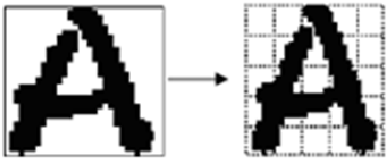
\includegraphics[width=\linewidth,height=30mm]{img/textDetection/feature_zoning.png}
\caption{Zoning} \label{fig:1b}
\end{subfigure}
\hspace*{\fill} % separation between the subfigures
\begin{subfigure}{0.30\textwidth}
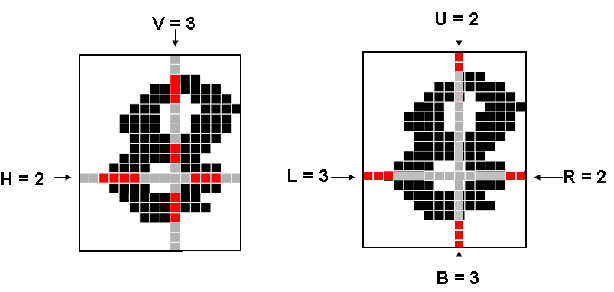
\includegraphics[width=\linewidth,height=30mm]{img/textDetection/feature_crossing.png}
\caption{Crossing and distances \citep{crossingAndDistances}} \label{fig:1c}
\end{subfigure}
\begin{subfigure}{0.30\textwidth}
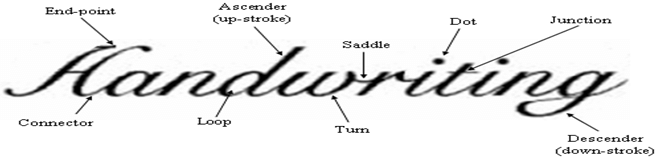
\includegraphics[width=\linewidth,height=30mm]{img/textDetection/features_geometrical.png}
\caption{Example of a few geometrical and topological features \citep{geometricalFeatures}} \label{fig:1c}
\end{subfigure}
\caption{Examples of feature extraction techniques} \label{fig:1}
\end{figure}


\subsection{Character classification}
\todo{Trosku problem je, ze na relativne jednoduchy metody pripravy textu spotrebujes 15 stranek a o hledani a klasifikaci pismen mas 1 sekci.}

OCR engines widely use the methodologies of pattern recognition, which assign an unknown sample into one of its predefined classes. There exist various approaches dealing with these methods, which are not necessarily independent of each other. Most often than not, OCR engines combine multiple methods to achieve the most accurate results.

One way to approach classification is by \emph{Template Matching} \citep{templateMatching}. It is based on the existence of predefined \emph{templates} --- multiple bitmaps containing characters of the alphabet. Improved version of this method have an extended database of templates, including numbers and special characters. Once a character is detected, it is passed to the algorithm and for every existing template, its similarity ratio is calculated. The template with the greatest ratio is then assumed to be the recognized character. This method has various implementation depending on how the ratio is calculated --- for example cross correlation, normalized correlation or euclidean formula can be used.

Although the implementation of this method is very simple, even small disfigurements and noise can greatly affect its efficiency. Also, in this case, a feature extraction would be unnecessary as all templates are created manually.

\begin{figure}[t]
    \noindent
	\makebox[\textwidth]{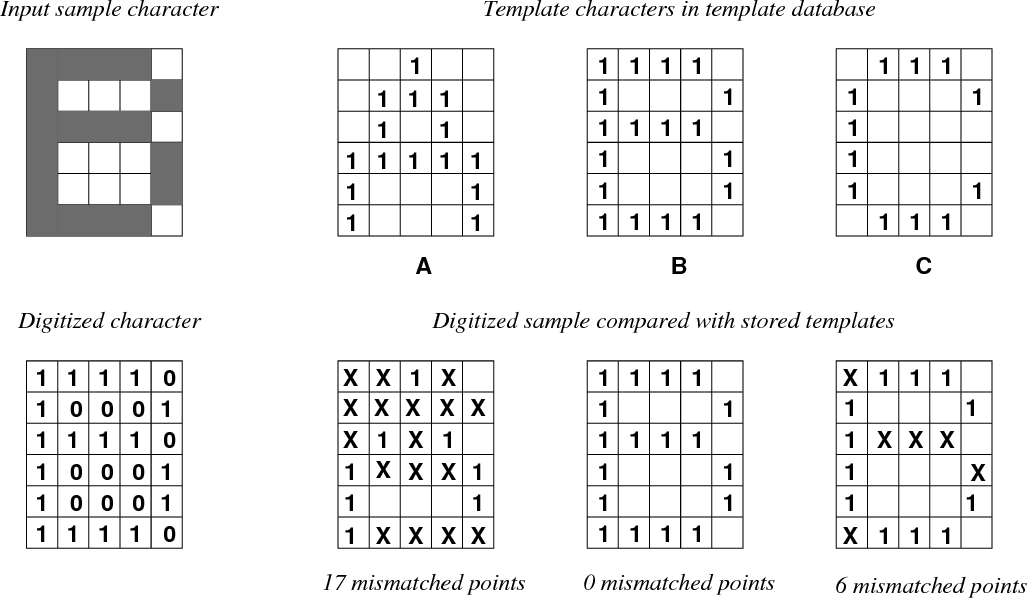
\includegraphics[width=30em]
	{img/characterClassification/templates.png}}
	\caption{Examples of template matching technique as described by \citet{Ning1993AnIO}}
	\label{fig:mff}
\end{figure}

Another approach is by using \emph{statistical techniques}~\citep{characterClassification} that also make use of the previous steps mentioned in this thesis. They are based on statistical modeling of the data. To determine the output, extraction of the features from input image (such as size, shape, intensity) is first performed. Then, with the help of statistical decision functions, these features are compared to the statistical model. The problem with these algorithms is that they have no information about whole-part relations. 

\begin{figure}[H]
\begin{subfigure}{0.30\textwidth}
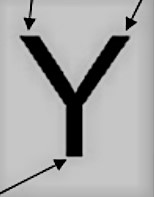
\includegraphics[height=10em]{img/characterClassification/statis_endPoint.jpg}
\caption{Existence and number of end points} \label{fig:1b}
\end{subfigure}
\hspace*{\fill} % separation between the subfigures
\begin{subfigure}{0.30\textwidth}
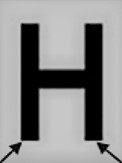
\includegraphics[height=10em]{img/characterClassification/statis_vertical.jpg}
\caption{Number of vertical lines} \label{fig:1c}
\end{subfigure}
\hspace*{\fill} % separation between the subfigures
\begin{subfigure}{0.30\textwidth}
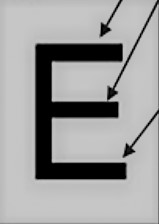
\includegraphics[height=10em]{img/characterClassification/statis_horizontal.jpg}
\caption{Number of horizontal lines} \label{fig:1c}
\end{subfigure}
\caption{A few of the possible extracted features in statistical techniques \citep{vithlani2015structural}} \label{fig:1}
\end{figure}

For this reason, a newer approach has been tested out over the past few years - \emph{machine learning} \citep{characterClassification}.

\emph{Machine Learning} \citep{sebastiani2002machine} is a method of data analysis based on artificial intelligence. Over time, it builds models of "training data". Based on them, it makes decisions and predictions on its input. 

In the case of character classification, training data is created by passing various characters into the engine and also providing it with the correct output. In this way, the engine learns how different characters should look and applies this knowledge to its input.

This method is for example used in a one of the simplest machine learning algorithms, and that is the \emph{KNN Classification Algorithm}, or K-Nearest Neighbor algorithm. The input image is compared to the training data and chooses its K nearest objects (objects that are the most similar). After that, the image is classified with being assigned to the class most common among its K nearest neighbors.

\begin{figure}[t]
\centering
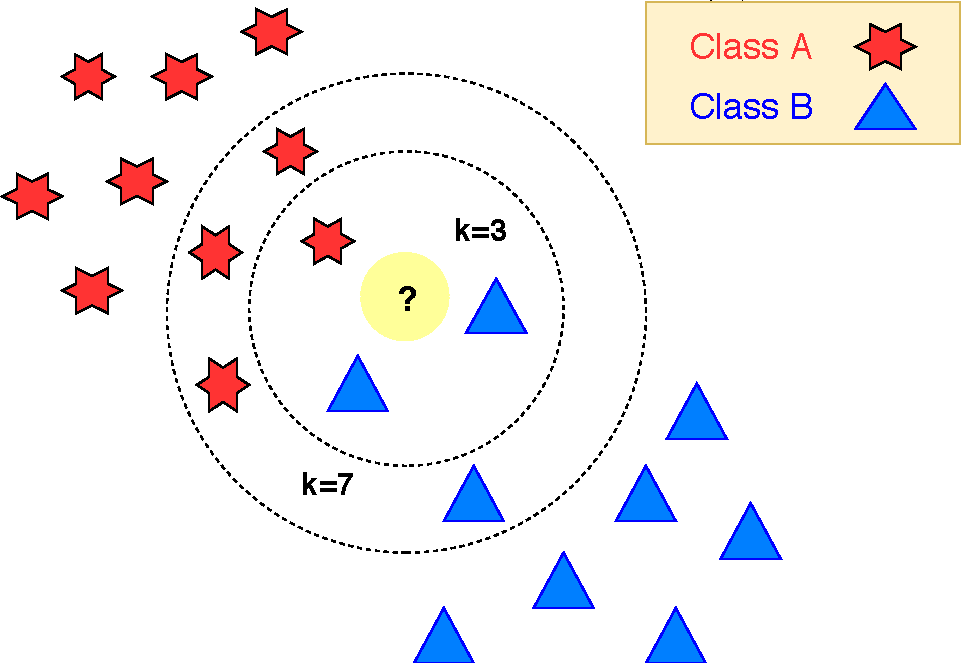
\includegraphics[width=0.7\linewidth]{img/characterClassification/knn.pdf}
\caption{KNN algorithm: with k=3, the algorithm will assign the new element to class A; wth k=7 to class B } \label{fig:1a}
\end{figure}

More complex methods include the \emph{Support Vector Machine algorithm} (SVM). This approach divides the data received into two classes --- training and testing data. The goal of SVM technique is to deliver a model that predicts the output of the test set.

The learning is done by a \emph{SVM kernel}. The kernel is, briefly speaking, a combination of mathematical function that takes two inputs and returns an information about how similar they are. Other than kernel functions, there are other parameters that tune the output of the SVM algorithm --- \emph{margin} parameter tells the engine the separation of line to the closest class points, \emph{gamma} parameter decides how far the influence of a single training example reaches and \emph{regularization} parameter controls the misclassification of elements.

\begin{figure}[H]
\centering
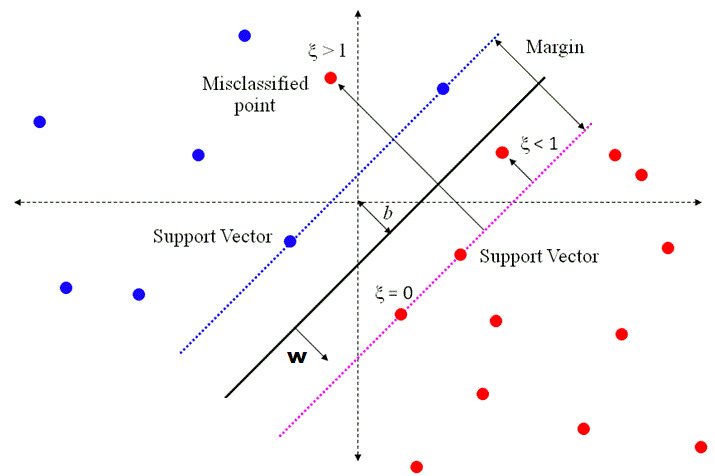
\includegraphics[width=0.7\linewidth]{img/characterClassification/svm.jpg}
\caption{The process of determination of classes in SVM algorithm \citep{svmAlgorithm}} \label{fig:1a}
\end{figure}

Many experiments have been executed in the field of machine learning for character classification. However, none of them can guarantee the accuracy of different approaches, as they all greatly depend on the training data. The more training data the machine can get, the more accurate it is. 

\section{Available OCR software}

Over the past few years, the demand for reliable OCR engines has risen, which lead to many new implementations and improvements of the already existing ones.

In this section, we present the overview of the most popular OCR engines. We also 

Most people take the expression "optical character recognition" to mean solely text recognition. This term, however, has a wider meaning - it also includes the recognition of other document elements, like images, forms, tables and many more.

There exist few OCR engines that provide all the features an OCR software should have - such as different types of preprocessing, support for all file extensions, recognition of different fonts, including handwritten documents. This is not needed in most cases. For example, customers using OCR for ticket validation do not need to process handwriting or different fonts, and customers trying to achieve automatic number plate recognition do not need to process tables or forms or any other elements.

For this purpose, a lot of OCR engines focusing entirely on one or more cases were implemented, as it is less complicated, time consuming and does the job. However, all of these existing OCR engines, no matter how difficult, have one thing in common - they all have to recognize text elements to some extent.

It this chapter, we will be concerned with the most popular and widely used OCR engines that focus (among other things) on word and character recognition. We will also discuss engines used for the preprocessing part of the algorithm.

\subsection{Tesseract}

Originally developed by Hewlett-Packard Company around 1990 \citep{TesseractGIT}, Tesseract is one of the most robust and accurate open-source OCR engines. When it was firstly developed, Tesseract could only accept TIFF images containing simple one-column text in English language. Since then, it has undergone a lot of improvements and added many features. As of today, Tesseract supports multi-columned documents (via its page-layout analysis), claims to support over 100 languages (including right-to-left text such as Arabic or Hebrew), works on different input and output image formats (with the help of Leptonica \citep{LeptonicaLIB} library) and is available for Windows, Linux and even Mac OS. In its latest version (4.0.0), Tesseract also added a new neural network (specifically a LSTM network) focused on line recognition. 

Tesseract does not have a GUI and works as a command line program. It is used mostly for development purposes and provides an OCR engine (libtesseract) that gives developers a chance to create their own applications using tesseract API. Also, Tesseract contains no preprocessing algorithms. It advises users preprocess the input images themselves \citep{TesseractQual}.

This is the reason why many wrappers and other 3rd party projects using Tesseract have been created. These projects mostly focus on creating GUIs for Tesseract or adding preprocessing algorithms to make the Tesseract engine more user-friendly. Although Tesseract is still in the process of development, it plans on doing no such thing and its future work consists mainly on focusing on LSTM networks.

Tesseract is one of the few OCR open-source engines. That is why it is so widely used for development and research purposes. However, for quick, everyday and user-friendly purposes, this is not the choice to go with.

\subsection{OpenCV}

OpenCV is an open source computer vision and machine learning software library. It claims to have more than 2500 optimized algorithms used for face detection and recognition, 3D object manipulation, photography editing (like red eye removal), tracking of moving objects or camera movements and other image processing functions \citep{OpenCV}.

On contrary to Tesseract, OpenCV is a user-friendly library. It is widely used as a framework for creating OCR applications and contains a lot of preprocessing functions. These can be then passed to the recognition algorithm, which makes the whole process of recognition easier and simpler. However, its main area of expertise is not OCR and definitely not document manipulation. For recognition, it mostly applies the \emph{template matching} technique. This technique is simple and easy to implement and works very well on ticket validation, credit card recognition or car plate recognition. Although these are all areas that OpenCV is widely used for with great success rate, the outputs from text document OCRs are poor [ref? to find]. It does not even have a library specialized for OCR.

The reason for mentioning OpenCV is exactly for its vast variety of preprocessing options. There are many projects that incorporate the work of OpenCV and Tesseract to achieve the most accurate and, most importantly, user-friendly results. Although OpenCV is mostly used via its Python interface, it also has a C++ and Java interfaces which can connect with Tesseract either directly via its C++ API, or through a wrapper like PyTesseract.

 However, these programs have almost no value for developers (except for comparison studies), whose work is still either concentrated on improving and expanding the Tesseract engine, or based on Tesseract's robust library.
 
 